\chapter{Etat de l'art sur le thème environnement-santé} \label{Art}

Sans être exhaustifs, nous relatons ici, les principes relatifs au thème environnement-santé appliqué au paludisme, puis un rapide survol des logiciels et chaînes de traitements existants traitants d'indicateurs de risque épidémiologique.

\section{Interactions environnement-santé}

Je me suis focalisé dans un premier temps sur la définition des facteurs de risque de transmission dans le contexte des interactions environnement-santé et plus précisément dans le contexte de la maladie du paludisme. Dans une première partie les termes pertinents pour ce travail sont définis. Par la suite sont expliqués de façon détaillée les facteurs de risques de transmission identifiés à partir d'une recherche bibliographique.

\subsection{Définitions}


\subsubsection{Approche environnement-santé}

L'approche environnement-santé s'intéresse à l'influence de la qualité de l'environnement physique, chimique et biologique sur la santé des hommes et des animaux d'un point de vue spatial et dynamique. Il s'agit donc d'une science dont les frontières sont extrêmement difficiles à délimiter tant les domaines couverts sont  potentiellement vastes et susceptibles d'interférer les uns avec les autres \citep{afsset2006}.

\subsubsection{Paludisme}
Le paludisme, appelé également malaria, est une parasitose due à un protozoaire transmis par la piqûre de la femelle d'un moustique (\textbf{anophèle}), provoquant des fièvres intermittentes. Le paludisme est la maladie vectorielle la plus commune dans le monde avec une estimation de 216 millions de cas et 665000 décès en 2010 \citep{WHO2012} principalement dans les régions tropicales et en en Afrique sub-saharienne. Ces chiffres seraient bien inférieurs à l'étendue réelle de cette maladie, dont la mortalité est tout de même observée à la baisse grâce à l'action positive des programmes de contrôle (Murray et al, 2012).

Le médecin français Alphonse Laveran a découvert la cause de la maladie en 1880 à Constantine (Algérie). Le moustique anophèle se reproduit dans les zones marécageuses. Le parasite qui possède plusieurs hôtes intermédiaires, dans l'état endémique, infecte les cellules hépatiques de la victime puis circule dans le sang. Au cours de son cycle de vie, le parasite à l'intérieur de l'organisme humain, fait un certain nombre de transformations qui lui permettent d'échapper au système immunitaire humain. Au final, lorsqu'un moustique non-infecté pique une personne contaminée, le parasite est également transmis de l'homme au moustique.

En France et dans les autres pays développés, le paludisme a disparu depuis les années 1960. Malgré tout, depuis les années quatre-vingt les nombreux voyages effectués dans les pays où il est endémique, notamment dans les régions tropicales et subtropicales ont causé une réapparition de la maladie dans les pays développés.  

Actuellement, le paludisme est responsable de plus de 300 millions de cas de maladie aiguë et d'au moins un million de décès dans le monde. Quatre-vingt-dix pour cent des décès dus au paludisme surviennent en Afrique, au Sud du Sahara, principalement chez les jeunes enfants. De nos jours, aucun vaccin efficace n'a encore pu être développé et les scientifiques doutent de plus en plus qu'ils trouveront un jour la solution miracle contre cette maladie  \citep{questquelepaludisme}.

\subsubsection{Vulnérabilité}

La vulnérabilité dans le domaine de l'environnement-santé est la probabilité qu'une personne soit affectée (dans notre cas d'étude de la source d'une maladie) en fonction de sa susceptibilité aux effets de l'aléa et du niveau d'exposition. La précarité social et la vulnérabilité médicale sont étroitement associées et s'additionnent souvent \citep{DictionnaireSante}.

\subsubsection{Aléa}

Pour définir l'aléa pour le risque sanitaire, nous nous appuyons sur les travaux de \citep{Aschan2009}. Ces auteurs  définissent l'aléa comme une menace d'origine naturelle ou humaine sur un  système et distinguent deux  types d'aléas. Les perturbations sont des évènements ponctuels, repérables dans le temps, dont l'ampleur dépasse la variabilité habituelle du phénomène. Le « stress » est un autre type d'aléa qui exerce une pression continue sur le système, mais dont la variabilité est limitée.

\subsubsection{Risque}

Le risque peut être défini comme la combinaison entre l'aléa et la vulnérabilité. Le risque est la probabilité, aléatoire ou non d'un événement qui menace la santé ou met en danger la vie d'un individu ou d'une population. Le risque dépend de la capacité d'une population ou d'un système de faire face à des menaces (aléas). On peut distinguer des risques de nature différente: risques génétiques, risques naturels, risques anthropiques ou risques technologiques \citep{ORSN2010}.

En France et dans les pays de développement le paludisme a disparu parce que les responsables ont été capables de diminuer au minimum la vulnérabilité de la population et leur exposition au risque (en éradiquant les moustiques par exemple). 

D'autres notions associées au risque doivent être prises en compte dans l'analyse d'un risque sanitaire. La perception d'un risque donnée varie d'une personne à une autre, d'une société à une autre et conduit à des comportements protecteurs différents. Aussi l'enjeu du risque varie selon les personnes: être malade peut avoir des conséquences sociales et économiques graves pour un foyer, tout comme pour une société.

\subsubsection{Facteur de risque}
Un facteur de risque est la caractéristique individuelle ou collective, endogène ou exogène, augmentant de façon statistiquement significative la probabilité d'apparition et de développement d'une maladie. Un facteur de risque n'est donc pas une "cause". Il est également important de différencier facteur de risque et marqueur de risque (par exemple âge, sexe, groupe sanguin etc) car tout facteur de risque peut être contrôlé ou supprimé \citep{DictionnaireSante}.

Dans le cadre de cette étude, les facteurs de risques sont l'ensemble des éléments qui augmentent la probabilité que la  maladie (le paludisme) se développe sur un territoire. Un facteur de risque concerne donc aussi bien les aléas que la vulnérabilité. L'ampleur d'un risque , sa fréquence, sa durée, son aire d'extension et de diffusion éventuelle (espace à risque)à sont fonction de facteurs de risque.

\subsubsection{Indicateur}

Selon la norme ISO 8402, un indicateur est une "information choisie, associée à un phénomène, destinée à en observer périodiquement les évolutions au regard d'objectifs périodiquement définis". Un indicateur est donc une variable qui décrit un élément d'une situation ou une évolution d'un point de vue quantitatif. Un indicateur est un outil d'aide à la décision et n'a d'intérêt que par les choix qu'il aide à faire dans ce cadre \citep{ANAES2012}. 



\subsubsection{Carte de risque}

Une carte de risque permet de visualiser les zones de risque principales face à un "risque" spécifique. Une carte de risque est généralement obtenue en combinaison des cartes de vulnérabilité (par exemple densité de population) et des cartes d'aléas (par exemple proximité d'une surface d'eau ou de végétation dans le cas du paludisme). Ces cartes permettent, dans le futur, d'aménager le territoire de façon plus adapté au risque et de savoir par exemple, quels quartiers d'une ville sont particulièrement exposés à un risque. Une carte de risque permet de présenter de façon synthétique les risques. De telles cartes doivent être prudemment interprétées et utilisées et ne pas être distribuées sans explications. La façon de présenter et de discrétiser les données dans une carte peut conduire à de mauvaises interprétations.


\subsection{Facteurs de risque de transmission du paludisme}

En me basant sur une recherche bibliographique, j'ai élaboré une liste des différents facteurs causant respectivement le développement et la transmission du paludisme et qui sont susceptibles d'agrandir la vulnérabilité des habitants sur un territoire. Les facteurs peuvent être les mêmes pour d'autres maladies climato-dépendantes. Les facteurs sont regroupés en 3 catégories: Les facteurs liés à l'environnement, les facteurs biologiques et les facteurs humains. Les facteurs jouent un rôle plus ou moins important dans le développement du paludisme. Pour chaque catégorie un tableau présentera les différents facteurs. Chaque facteur sera par la suite expliqué en détail afin d'illustrer les caractéristiques spécifiques à chaque facteur de risque.

\newpage
\subsubsection{Facteurs environnementaux}
Les facteurs environnementaux sont en lien direct avec par exemple les conditions météorologiques ou avec la morphologie des sols sur un territoire. Toutes ces conditions vont influencer le risque que le paludisme puisse être transmis sur un territoire. \\

\begin{center}
\begin{tabular}{|c|c|} 
\hline
\textbf{Numéro} & \textbf{Facteur}\\
\hline
1 & Précipitation\\
\hline
2 & Température\\
\hline
3 & Distance au point d'eau le plus proche\\
\hline
4 & Caractéristiques du point d'eau\\
\hline
5 & Altitude\\
\hline
6 & Humidité\\
\hline
7 & Humidité du sol \\
\hline
8 & Température mois précédant les précipitations\\
\hline
9 & Végétation\\
\hline
\end{tabular}
\end{center}


\paragraph{Précipitation:}
Les précipitations sont parmi les facteurs de risque les plus important du paludisme puisqu'elle conditionnent l'écologie des moustiques, vecteurs des parasites. En examinant des territoires avec des cas de paludisme et des territoires sans cas de paludisme, il faut qu'il pleuve pendant 3 à 5 mois au moins 80 mm par mois pour que le paludisme puisse se développer \citep{Adjuik1998}. Les précipitations créent également des points d'eau temporaires, souvent difficilement repérables et idéaux pour le développement des moustiques. Ces points d'eau temporaires sont généralement de bonne qualité (non-pollués), ce qui est un autre facteur important.

\paragraph{Température:}

Le pourcentage de survie des moustiques sur un territoire est étroitement lié à la température \citep{Ermert2011}. Les moustiques disparaissent à partir d'une température de moins de 5°C et ne supportent pas des températures supérieures à 40°C. D'autres expériences montrent également que les moustiques ne peuvent pas survire les 56 jours de leur cycle de reproduction normal si les températures sont inférieures à 16°C et/ou supérieures à 32°C. La température idéale pour le cycle de reproduction du moustique est de 22°C. Dans ce cas-là, le cycle est fini après seulement 22 jours. \citep{Adjuik1998}

\paragraph{Distance point eau} 

Les moustiques anophèles peuvent se déplacer d'un maximum de 7 kilomètres par rapport à un point d'eau \citep{Ermert2011}. Les hommes habitant à plus de 7 kilomètres d'un point d'eau (de bonne qualité) ne sont donc, en théorie, exposés à aucun risque de paludisme. Néanmoins il est plutôt rare, notamment dans les pays en développement et donc dans les zones de risque majeures du paludisme que les gens habitent aussi éloigné d'un point d'eau. En plus, des expériences ont démontré que les moustiques infectés du paludisme peuvent être amenés par des voitures (par exemple) dans des zones non-vulnérables auparavant.

\paragraph{Caractéristiques du point eau} \label{caracteaux}
La surface et surtout la turbidité de l'eau jouent un rôle non négligeable dans le développement du paludisme. Lorsque le courant est trop fort, les œufs des moustiques sont lavés, les moustiques ne peuvent donc pas se reproduire. 
Des essais en laboratoire \citep{Minakawa1999} ont montré que les moustiques anophèles pondent plus d'œufs dans les points d'eau se situant sur des sols inondés ou humides que dans de l'eau "sans sol". En plus, les moustiques anophèles n'aiment pas, en général, les habitats ombragés tels que des réservoirs d'eau sans substrats de sol. En effet, le sol fournit des éléments nutritifs qui favorisent l'accumulation de bactéries qui sont la source de nourriture pour les larves.

\paragraph{Altitude}
L'altitude maximale retenue généralement est de 2000m. Ce facteur est bien évidemment étroitement lié au facteur de la température car la température diminue de 0.7°C tous les 100 mètres.

%\paragraph{NDVI}
%
%Le NDVI (normaized difference vegetation index) intègre et combine les effets de la température, humidité, précipiations et de l'altitude. Le NDVI varie entre -1 et +1 et se base sur l'optimum de...
%Rechercher définition scientifique.

\paragraph{Humidité de l'air}
L'humidité relative de l'air a un impact important sur la présence et la persistance des sites de reproduction des moustiques. Le taux de survie des moustiques est également influencé par ce facteur.

Le facteur peut être extrait à partir d'autres facteurs météorologiques comme les précipitations et la température mais doit être utilisé avec précaution . L'humidité est fortement influencée par la température de l'air et peut donc significativement changer pendant un seul jour. A noter que ce facteur dépend également de l'altitude. L'humidité idéale pour les moustiques est de 60 \% \citep{Protopopoff2009}.


\paragraph{Humidité du sol}
L'humidité du sol dépend directement des températures, de la végétation ou de la présence de points d'eau. Ce facteur est particulièrement intéressant car il peut être extrait à partir des images satellites. \citep{Machault2011}

\paragraph{Végétation:}

Certains types de végétation servent comme habitat pour les moustiques adultes.\citep{Minakawa1999} (à revoir)

\newpage

\subsubsection{Facteurs biologiques = marqueur de risque}

Les facteurs de risque de transmission biologiques sont liés par exemple à l'organisme humain ou à l'organisme du moustique. L'état de l'organisme humain, sous certaines conditions, peut augmenter le risque de l'apparition du paludisme sur un territoire. Certains de ces facteurs comme l'âge sont également des marqueurs de risque et ne peuvent pas être influencées respectivement modifiées.\\

\begin{center}

\begin{tabular}{|c|c|} 
\hline
\textbf{Numéro} & \textbf{Facteur}\\
\hline
1 & Etat de santé de la personne\\
\hline
2 & Densité du vecteur\\
\hline
3 & Transmission Homme-Moustique\\
\hline
4 & Immunité\\
\hline
5 & Age \\
\hline
\end{tabular}
\end{center}

\paragraph{État de santé de la personne}

L'état de santé de la personne joue un rôle majeur dans le développement du paludisme. Les personnes les plus en risque sont les enfants de moins de trois ans et les femmes enceintes et donc les personnes avec les systèmes immunitaires les plus fragiles. Les adultes ou les adolescents présentent généralement des systèmes immunitaires suffisamment puissants pour combattre le paludisme. 
\citep{Protopopoff2009}

\paragraph{Densité du vecteur}

Pour combattre le paludisme, il n'est pas nécessaire d'éradiquer complètement les moustiques sur le territoire mais il suffit de réduire la densité vectorielle \citep{Gaudart}. En général, la densité de l'anophèle diminue avec l'éloignement du gîte, avec la densité du tissu urbain et de la périphérie vers le centre \citep{Gaudart}. En analysant les densités vectorielles sur différents territoires, il est possible de déterminer les végétations ou écosystèmes les plus favorables pour le développement des larves.

\paragraph{Transmission Homme-Moustique}

En cas de piqûre, un humain porteur du parasite du paludisme transmet la maladie aux moustiques non-infectés par avant. Ceci est un autre facteur de risque à ne pas négliger, le taux de transmission est de 20\% (30\% pour une transmission moustique-homme).

\paragraph{Immunité} \label{immunite}
La capacité d'un organisme humain pour combattre l'infection du paludisme dépend de son immunité \citep{Protopopoff2009}. A partir de 2 à 3 ans, l'organisme humain développe et augmente l'immunité indépendamment du nombre de piqûres. Dans des régions avec peu de piqûres, le nombre de cas cliniques et d'infection est le même pour tous les groupes d'âge. Il faut donc que l'homme soit piqué régulièrement afin de développer une certaine immunité contre l'infection du paludisme.

\paragraph{Age}
Les enfants de moins de 3 ans sont piqués plus souvent, il semble que la proportion entre piqûres et un être humain soit liés à la taille du corps de l'hôte.  \citep{Ermert}

\subsubsection{Facteurs humains}
Les facteurs humains sont les facteurs liés à la présence humaine sur un territoire qui augmentent la vulnérabilité des habitants du territoire par rapport à la transmission du paludisme.

\begin{center}

\begin{tabular}{|c|c|} 
\hline
\textbf{Numéro} & \textbf{Facteur}\\
\hline
1 & Urbanisation \\
\hline
2 & Agriculture \\
\hline
3 & Qualité système santé \\
\hline
4 & Croissance démographique et Facteurs socio-économiques \\
\hline
\end{tabular}

\end{center}


\paragraph{Urbanisation}
L'urbanisation généralement diminue le risque du paludisme. Les points d'eau sont pollués, il y a peu de végétation etc. Ceci dépend malgré tout de la taille de l'urbanisation. Forcément, dans une grande ville le risque d'être piqué est moins grand car il y plus de "cibles" pour les moustiques, en même temps de nouveaux facteurs de risques peuvent apparaître comme par exemple les lumières et télévisions étant une source d'attraction pour les moustiques.

\paragraph{Agriculture / Irrigation}

Les activités agricoles influencent directement le risque du paludisme. Par exemple, en irriguant régulièrement les terres agricoles, ces surfaces (=surface d'eau temporaires et de bonne qualité) deviennent des endroits idéaux pour les moustiques pour pondre des œufs. La déforestation joue également sur le risque du paludisme. Des études récentes ont démontré que des habitations terrestres (des hommes) se situant en altitude, construits après une déforestation étaient des sites de reproduction préférés par les moustiques.\citep{Krefis2011}

\paragraph{Qualité système de santé}

La qualité du système de santé ou l'accès au système de santé influe directement sur le risque du paludisme  \citep{Protopopoff2009}. Des traitements préventifs permettent de réduire le taux de morbidité des femmes enceintes et des enfants, qui généralement ont le système immunitaire le plus fragile.


\paragraph{Croissance démographique / Facteurs socio-économiques}

Le statut socio-économique d'un individu est également d'importance. Les personnes les plus prospères sont capables de mieux se protéger contre les moustiques que les personnes très pauvres. Aussi, le niveau d'éducation peut influencer le risque de paludisme, Sachant que souvent les  personnes n'utilisent pas les filets anti-moustiques mis à leur disposition car ils ne comprennent pas vraiment le risque d'être piqués et le risque de paludisme, le niveau d'éducation des habitants est  également à prendre en compte.

Le type d'habitat de l'homme joue également un rôle important. En fonction du type d'habitat, le moustique peut entrer plus ou moins facilement dans l'habitat et piquer l'humain. Certains types d'habitations (en fonction du type de construction) peuvent même servir comme lieu d'habitat aux moustiques.


\subsubsection{Alea et Vulnérabilité selon les facteurs}

Les différents facteurs peuvent être regroupés en deux catégories différentes: les facteurs liés à l'aléa et les facteurs liés à la vulnérabilité. Certains facteurs peuvent créer un aléa et une vulnérabilité en même temps. Par exemple, en irriguant des terres, les agriculteurs créent involontairement un aléa (en créant des points d'eau temporaires) et aggravent en même temps la vulnérabilité des habitants du territoire. La figure \ref{AleaVuln} récapitule quels facteurs peuvent être à la base d'un aléa et lesquels peuvent aggraver la vulnérabilité.\\

\newpage

\begin{figure}[H]
\begin{center}

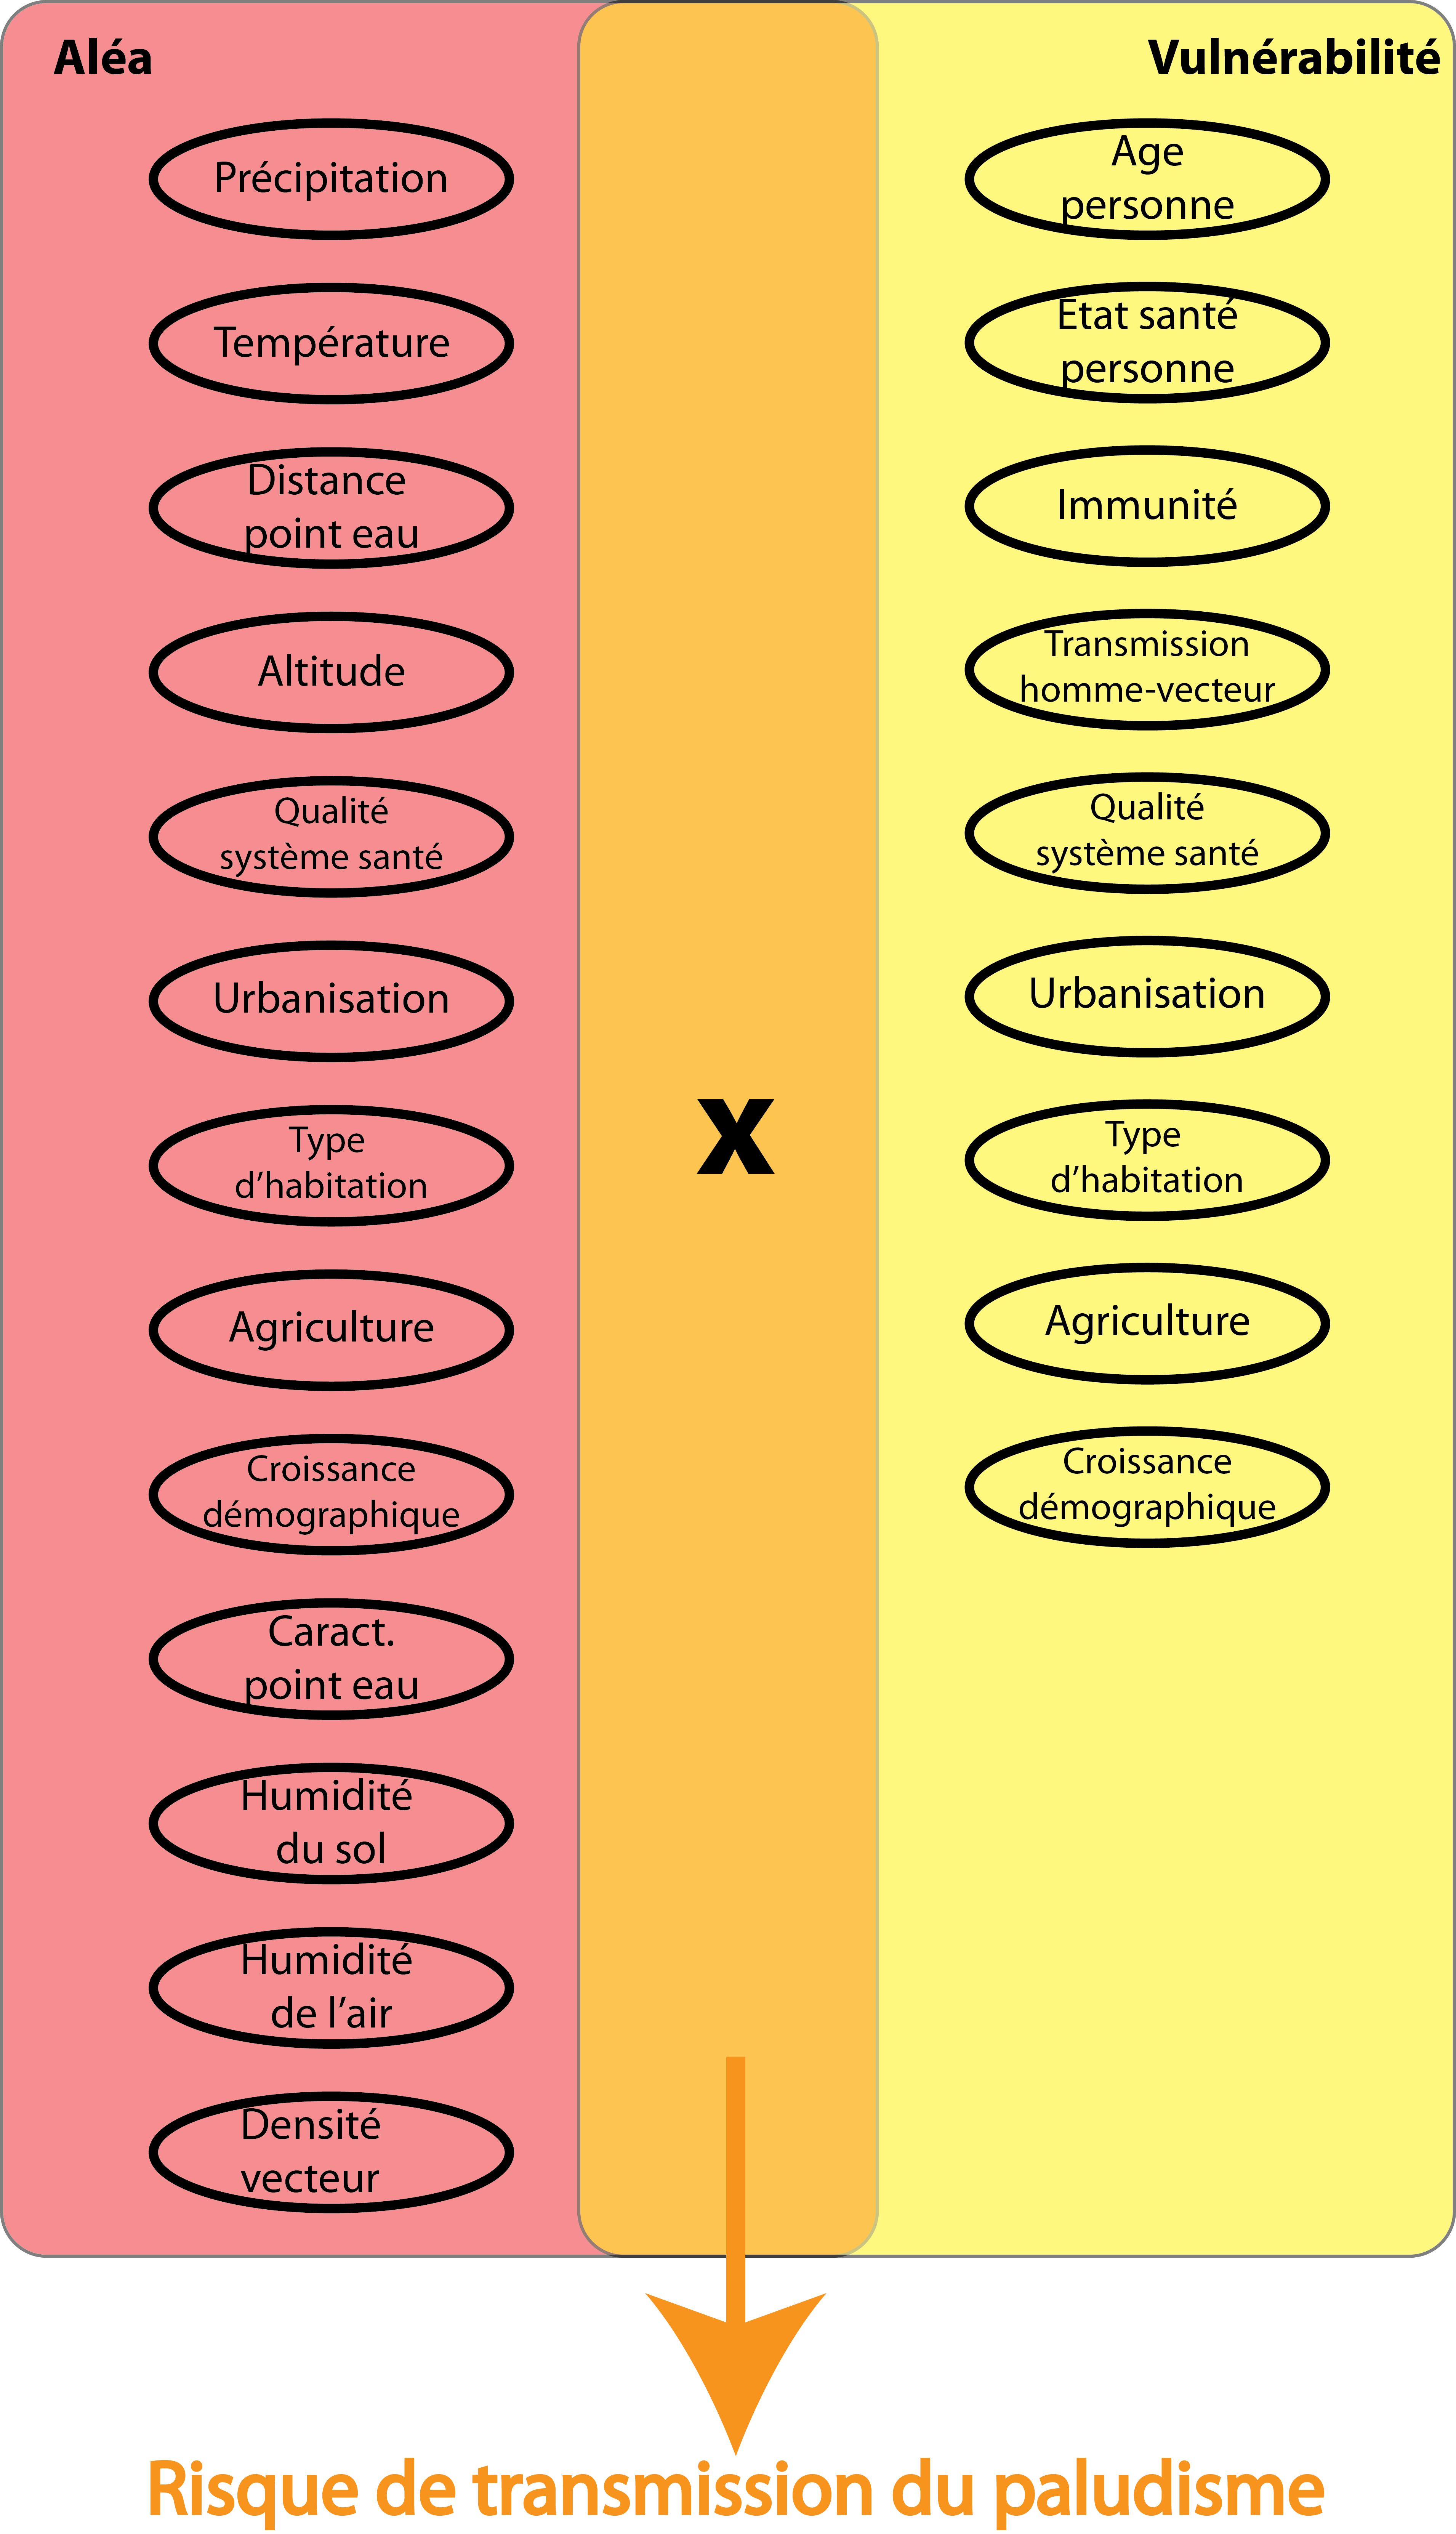
\includegraphics[width=9cm]{AleaVulnerab.png}\\
\caption{\label{AleaVuln} Alea et Vulnérabilité selon les facteurs}
\end{center}

\end{figure}


\section{Approches logicielles existantes}

Nous nous sommes simultanément intéressés aux logiciels et aux chaînes de traitements existants qui traitent les mêmes problématiques et / ou des problématiques similaires. Je présenterai dans cette partie du mémoire les approches logicielles que j'ai pu découvrir en faisant des recherches.

Nous avons focalisé nos recherches sur des outils qui se basent sur le principe d'analyse par rapport à l'existence de certaines variables (par exemple présence de points d'eau sur un territoire). Un autre principe d'analyse aurait été de définir le risque à travers l'absence de certaines variables (par exemple pas de végétation à proximité des lieux d'habitation des population).


\subsubsection{Repast Simphony}
Repast Simphony est une plate-forme de modélisation basée sur \textbf{Java}. Repast Simphony est un plugin \textbf{Eclipse} et permet de développer des programmes avec de nombreuses interactions. Repast Symphony a déjà été utilisé dans de nombreux domaines, comme en sciences sociales ou en sciences humaines. 


\subsubsection{Maxent}
Maxent est un logiciel gratuit qui permet de prédire la distribution potentielle (modélisation de l'habitat) des espèces animales ou végétales en se basant sur la distribution ponctuelle et certains facteurs environnementaux des espèces.

L'outil utilise comme variables d'entrée des données géoréférencées  des animaux respectivement de la végétation à modéliser et des données appropriées aux variables environnementales (par exemple pluviométrie, température, topographie etc.) au format ASCII (format ESRI). La modélisation est basée sur la méthode de l'entropie maximum. L'outil livre en tant que résultat une carte indiquant l'apparition potentielle des espèces ainsi que d'autres résultats statistiques. La visualisation des résultats se fait à l'aide d'un système d'information géographique. L'outil a été développé en Java et est disponible pour tous les systèmes d'exploitation.

\subsubsection{OpenModeller}

OpenModeller vise à fournir un environnement multi-plateformes permettant la réalisation de l'ensemble  du processus de "\textbf{niches fondamentales}". 
Le logiciel  facilite la lecture de l'occurrence des espèces et des données environnementales, la sélection des couches de données environnementales, la création d'un modèle de niche fondamentale et la projection du modèle dans un scénario de l'environnement. Un certain nombre d'algorithmes est également fourni sous forme de plugins et le logiciel permettant notamment de générer plusieurs modèles en utilisant différents
algorithmes face à une même problématique. Le projet est Open Source, multi-plateforme et développé en C++.


\subsection{Cas d'utilisation concret dans le contexte environnement-santé:}

\subsubsection{Le projet SimMasto}

Le projet SimMasto s'inscrit dans le cadre d'un projet de recherche sur la dynamique des populations de rongeurs. Il vise à développer une plate-forme générique de simulation des rongeurs dans leur environnement. Les données utilisées sont des cartes géographiques numériques, des cartes raster, des grilles théoriques etc.
La chaîne de traitements qui a été développée comprend les éléments permettant le traitement des images d'entrée (géoréférencement, détourage, changement de résolution, clipping, etc.) ainsi que tous les éléments de programmation nécessaires.

La chaîne de traitements est composée de plusieurs "modules", comme par exemple:
\begin{itemize}
\item Géoréférencement d'une image de type raster
\item Vectorisation d'une image de type raster (utilisation de la librairie Grass)
\item Modification du système de coordonnées
\end{itemize}

La chaîne de traitements fait par la suite appel à Repast Symphony pour mettre en place une simulation. Dans Repast Symphony est implanté un SIG, c'est-à-dire les différents fichiers de formes géoréférencés créés par avant ainsi qu'un fichier raster (une grille). D'autres outils / bibliothèques utilisés dans cette chaîne de traitements sont par exemples \textbf{PostgreSQL} / \textbf{PostGIS} ou \textbf{Eclipse}.


\section{Conclusion}

Dans le contexte choisi de l'environnement-santé, le premier travail a consisté à s'approprier la terminologie et à rechercher les outils logiciels existants.

Nous disposons des différentes définitions clairement établies, par contre sur le volet informatique, aucun outil ne semble proposer la solution attendue. En effet il n'existe pas, à notre connaissance et à ce jour, de chaîne de traitements automatisée permettant de cartographier facilement les zones de risque du paludisme. 

Il est donc particulièrement intéressant de proposer des prototypes d'outils permettant de cartographier les indicateurs relatifs à divers risques environnementaux. 

